\section{SySML Functional model}
In the picture \ref{fig:SystemComponents} is reported the functional Block Definition Diagram that describes the composition of the system, composed by one Central Unit and up to eight Rooms, the two modules are connected via two FlowPort as shown in \ref{fig:SystemInternals}.
The Central Unit send a \textit{RoomRequest} message composed as follows:
\begin{center}
	\begin{tabular}{||l | l| l ||} 
		\hline
		\textbf{parameter} 	& \textbf{type} & \textbf{[Min,Max]}\\ 
		\hline
		Id 					&  Natural & [1,8] \\ 
		\hline
		DesiredTemperature 	&  Float & [15.00, 30.00] \\ 
		\hline
	\end{tabular}
	\captionof{table}{Room Request variables \label{tab:RoomRequest}}
\end{center}
The Room module send a \textit{RoomStatus} message composed as follow:
\begin{center}
	\begin{tabular}{||l | l| l ||} 
		\hline
		\textbf{parameter} 	& \textbf{type} & \textbf{[Min,Max]}\\ 
		\hline
		Id 					&  Integer & [1,8] \\ 
		\hline
		Eco				 	&  Boolean & [0, 1] \\ 
		\hline
		Temperature			&  Float & [15.00, 30.00] \\ 
		\hline
		Humidity			&  Float & [0.00, 100.00] \\ 
		\hline
		Valve				&  Integer & [0, 100] \\ 
		\hline
	\end{tabular}
	\captionof{table}{Room Status variables \label{tab:RoomStatus}}
\end{center}

\begin{figure}[H]
	\centering
	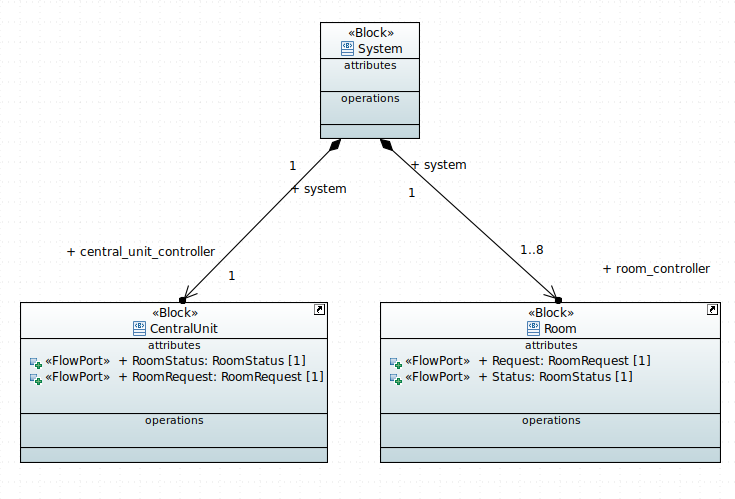
\includegraphics[width=12cm,keepaspectratio]{img/sysml/SystemComponents}
	\caption{System Components}
	\label{fig:SystemComponents}
\end{figure}
\begin{figure}[H]
	\centering
	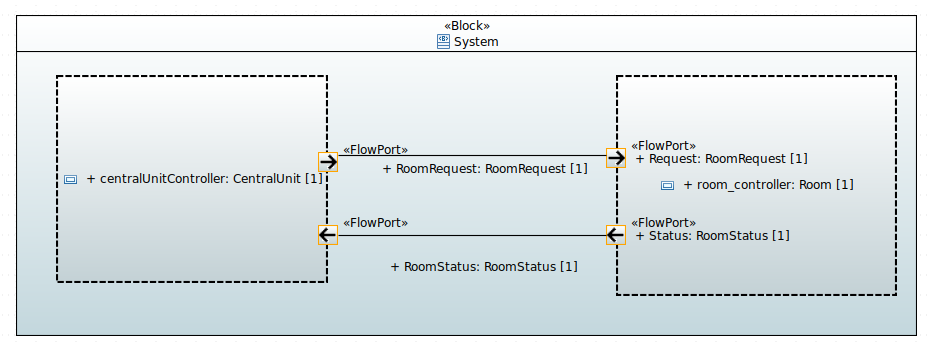
\includegraphics[width=12cm,keepaspectratio]{img/sysml/SystemInternals}
	\caption{System Internals}
	\label{fig:SystemInternals}
\end{figure}

\subsection{Central Unit}
The \textit{Central Unit} is composed by two modules, the \textit{RoomsManager} and the \textit{UserInterfaceManager}.
The \textit{RoomsManager} implements the functionalities related to the status of each room.
The \textit{UserInterfaceManager} that implements the functionalities related to represent the status of the system.
The two components exchange data as shown in \ref{fig:CentralUnit_internals}.
\begin{figure}[H]
	\centering
	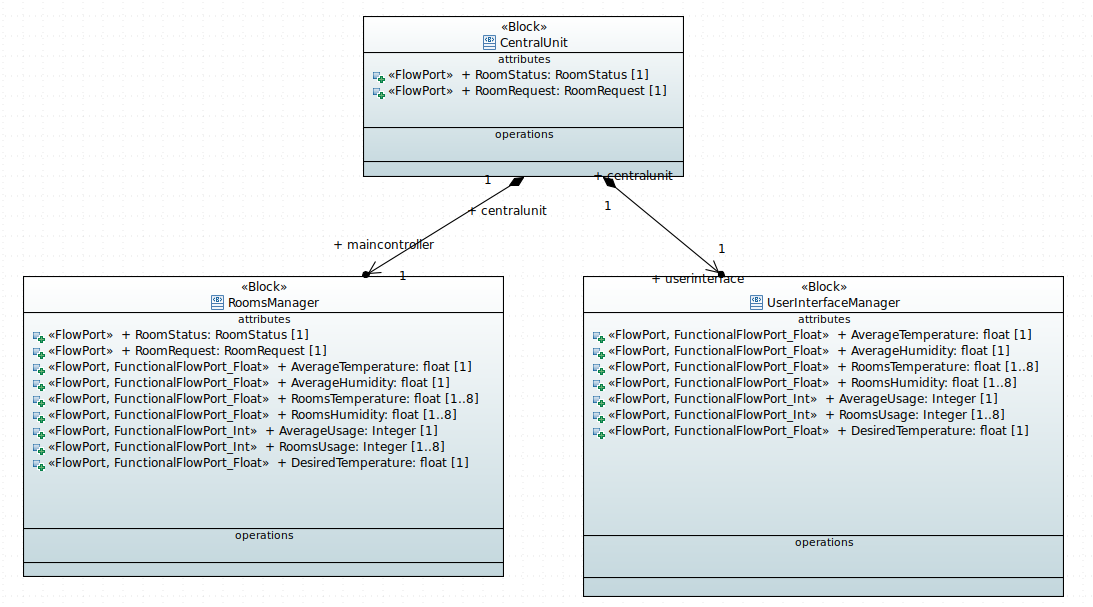
\includegraphics[width=12cm,keepaspectratio]{img/sysml/CentralUnitComponents}
	\caption{Central Unit components}
	\label{fig:CentralUnit_components}
\end{figure}

\begin{figure}[H]
	\centering
	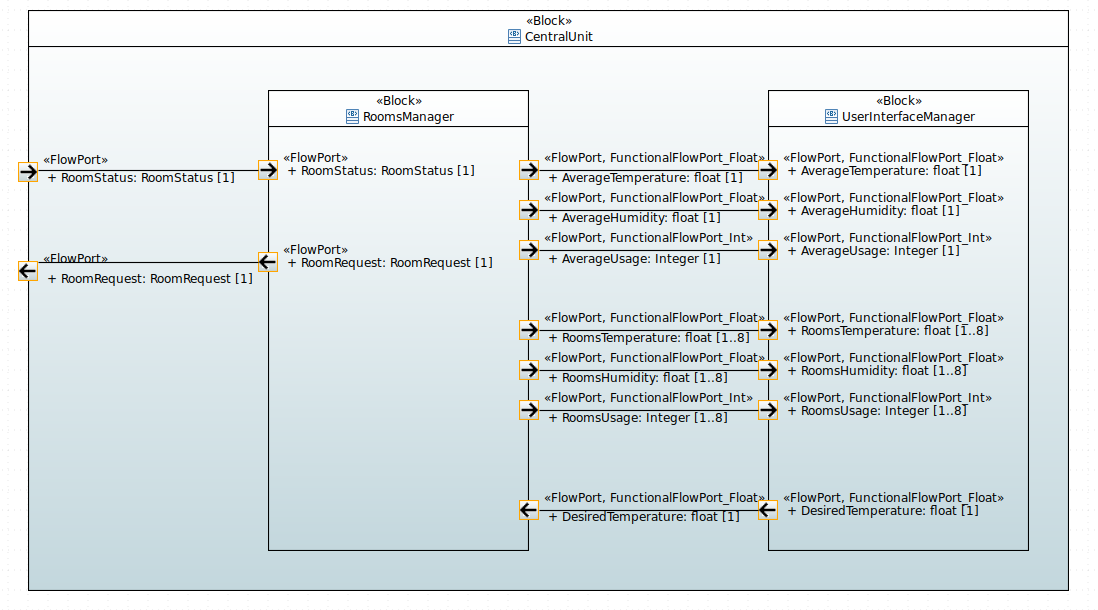
\includegraphics[width=12cm,keepaspectratio]{img/sysml/CentralUnitInternals}
	\caption{Central Unit internals}
	\label{fig:CentralUnit_internals}
\end{figure}


\subsection{Room module}
The main component of this module is the \textit{MainController} composed by different functions as shown in \ref{fig:RoomInternals}.
\begin{figure}[H]
	\centering
	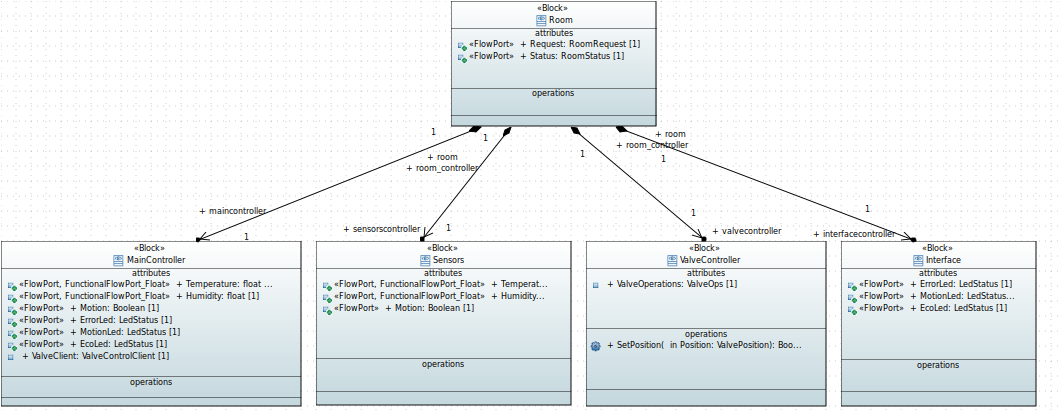
\includegraphics[width=13cm,keepaspectratio]{img/sysml/RoomComponents}
	\caption{Room Components}
	\label{fig:RoomComponents}
\end{figure}

\begin{figure}[H]
	\centering
	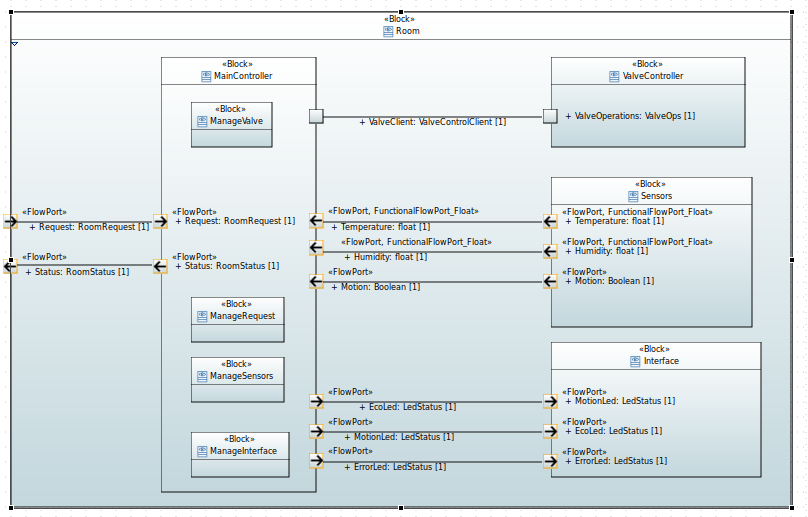
\includegraphics[width=13cm,keepaspectratio]{img/sysml/RoomInternals}
	\caption{Room Internals}
	\label{fig:RoomInternals}
\end{figure}

\begin{figure}[H]
	\centering
	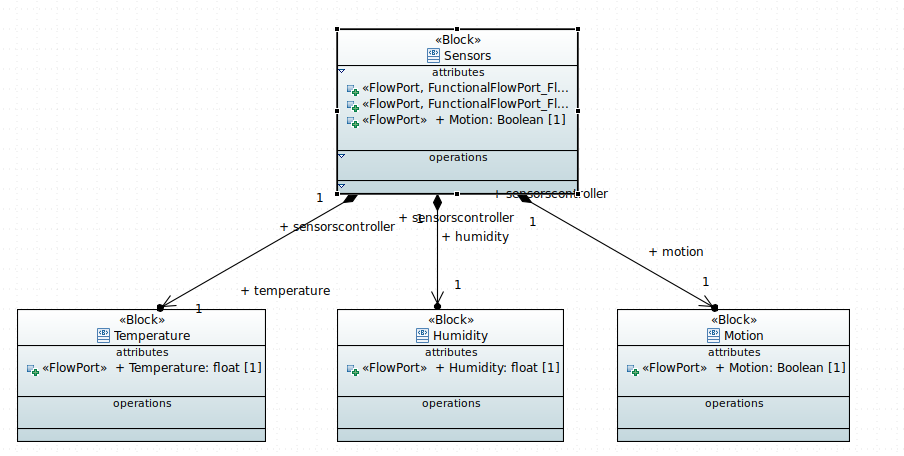
\includegraphics[width=13cm,keepaspectratio]{img/sysml/SensorsComponents}
	\caption{Room sensors components}
	\label{fig:room_sensors_components}
\end{figure}

\begin{figure}[H]
	\centering
	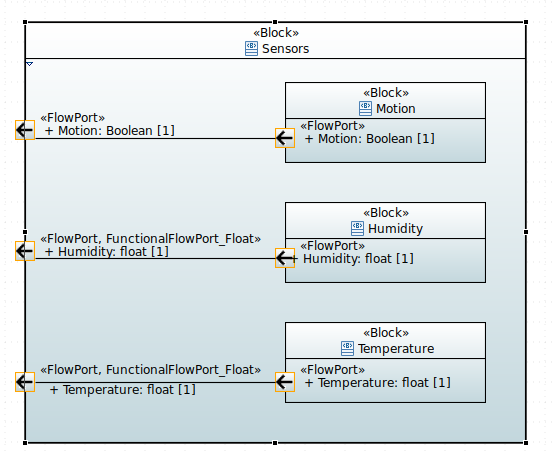
\includegraphics[width=8cm,keepaspectratio]{img/sysml/SensorsInternals}
	\caption{Room sensors internals}
	\label{fig:room_sensors_internals}
\end{figure}

\begin{figure}[H]
	\centering
	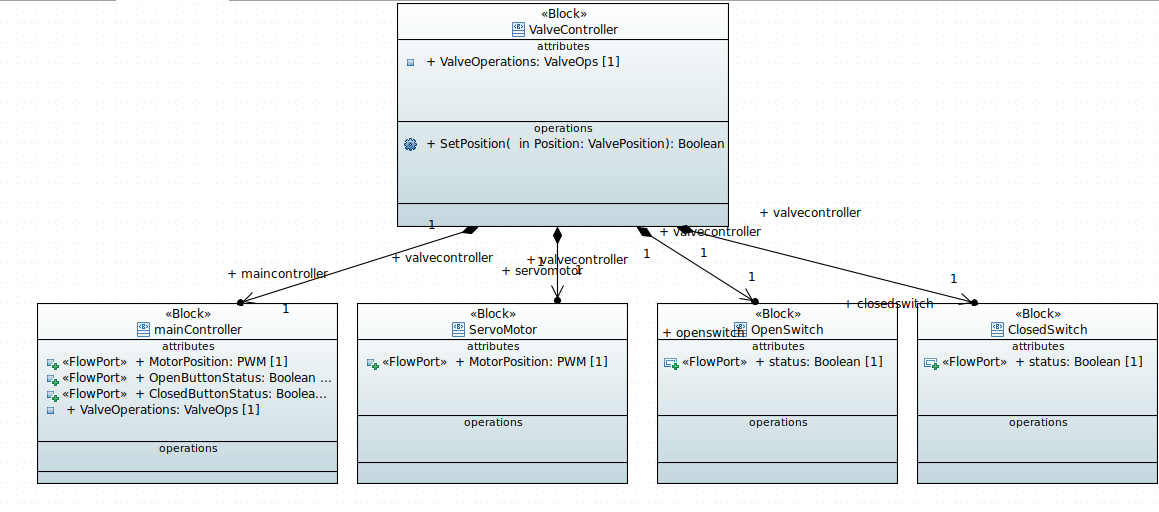
\includegraphics[width=12cm,keepaspectratio]{img/sysml/ValveControllerComponents}
	\caption{Valve Controller components}
	\label{fig:valve_dbd}
\end{figure}

\begin{figure}[H]
	\centering
	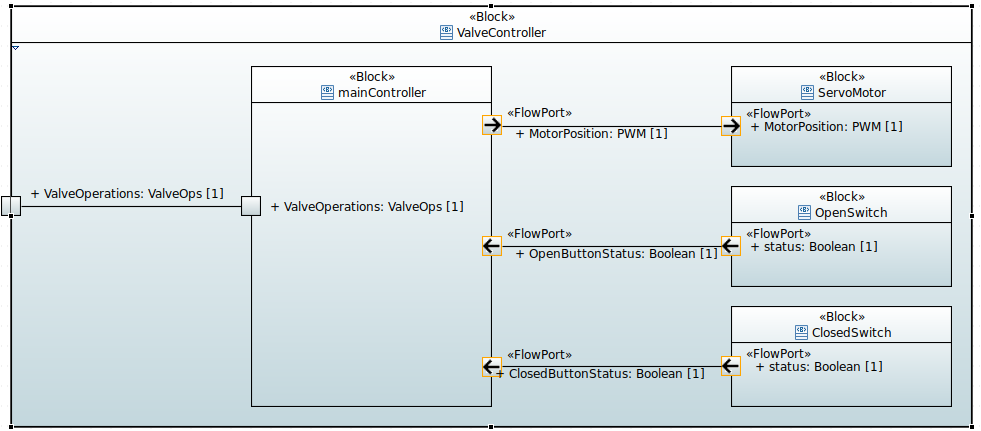
\includegraphics[width=12cm,keepaspectratio]{img/sysml/ValveControllerInternals}
	\caption{Valve Controller internals}
	\label{fig:valve_internals}
\end{figure}
